\documentclass[UTF8,a4paper,12pt]{ctexart}

\usepackage{amsmath,amssymb}
\usepackage{geometry}
\usepackage{array,tabularx}
\usepackage{enumitem}
\usepackage{fancyhdr}
\usepackage{tikz}
\usepackage{lastpage}
\usepackage{xurl}
\usepackage{float}
\usepackage{xeCJKfntef}
\usepackage[colorlinks=true, linkcolor=black, urlcolor=black]{hyperref}

\geometry{
  left=2.2cm,
  right=2.2cm,
  top=1.8cm,
  bottom=1.8cm
}

\setlength{\parindent}{0pt}
\setlength{\parskip}{0.5em}

\pagestyle{fancy}
\fancyhf{}
\renewcommand{\headrulewidth}{0pt}
\cfoot{\zihao{-5}第~\thepage~页~~共~\pageref{LastPage}~页}

\newcommand{\blank}[1][3cm]{\underline{\hspace{#1}}}
\newcommand{\fillblank}[2]{\underline{\makebox[#1][c]{#2}}}
\newcolumntype{C}[1]{>{\centering\arraybackslash}m{#1}}

\begin{document}

\thispagestyle{empty}

\begin{center}
    {\heiti\zihao{3} 说明}
\end{center}

\vspace{2em}

本份 DSP 期末试卷由 Fishplate 与一众志同道合的伙伴们整理制作。内容全部来源于笔者参加2026年的数字信号处理期末考试中的回忆。由于笔者几乎不可能在不借助任何外力的情况下回忆起所有细微数据、题目措辞、分值分配、题号等细致的内容。因此小部分题目笔者只能在\textbf{\CJKunderline{不改变题目考查内容与方向的前提下}}，人为推测编造一些数据、选项排布、分值。此外，本试卷也尽量还原了原试卷的排版。不过鉴于\LaTeX{}和Word文档排版方式的差异，只能做到尽量还原，请各位见谅。

\vspace{1em}

需要说明的是，本文档中的参考答案由 ChatGPT 5.5 生成，限于精力，本人无法逐题仔细核查。因此答案仅供复习参考，不保证完全正确。如发现题目或答案存在问题，欢迎自行修改、校对和完善。

\vspace{1em}

在这里十分感谢 Godknows、竹木、vespergraine 等同学的大力支持。没有你们提供的考后回忆、题目细节和交叉印证，笔者很难在考试结束后还原出这份残卷。

\vspace{1em}

也感谢所有参与讨论和补充的同学。由于本试卷本身来源于考后回忆，许多题目的数据、选项和表述都需要反复确认、推敲和重构。本文档能够最终整理出来为后人所用，离不开大家的共同努力。


\begin{center}

{\heiti{功成不必在我，功成必定有我！}}

\end{center}


本试卷开源至 GitHub：\url{https://github.com/Pandamonic/CUC_2025-2026_DSP_Final_Exam}，供同学们自由学习、复习和二次整理使用。如果发现有错误也欢迎大家在这里改正。

\vspace{1em}


\begin{center}

{\heiti{祝大家复习顺利，考试取得好成绩!}}

{\textbf{Per Aspera Ad Astra!}}

\vspace{1em}

{\heiti btw重要的事情说三遍：}

\vspace{1em}

{\heiti 本资料是免费的，如果你是花钱买到的，说明你被坑了！！}

{\heiti 本资料是免费的，如果你是花钱买到的，说明你被坑了！！}

{\heiti 本资料是免费的，如果你是花钱买到的，说明你被坑了！！}

\end{center}

\vfill

\begin{center}
Fishplate\\
\today
\end{center}

\newpage

\begin{center}
    {\heiti\zihao{4} 中国传媒大学}\\[0.8em]
    {\heiti\zihao{3} \fillblank{1cm}{2025}—\fillblank{1cm}{2026} 学年第\fillblank{1.1cm}{2}学期期末考试试卷}
\end{center}

\vspace{1.8em}

\begin{tabular}{@{}p{0.51\textwidth}p{0.43\textwidth}@{}}
考试科目：\fillblank{3.8cm}{数字信号处理}
&
课程编号：\fillblank{3.8cm}{2111030096}
\\[1.1em]
考试班级：\fillblank{3.8cm}{24级信通学院各专业}
&
考试方式：\fillblank{3.8cm}{闭卷}
\\[-0.2em]
&
\end{tabular}

\begin{center}
\renewcommand{\arraystretch}{1.55}
\setlength{\tabcolsep}{4pt}
\begin{tabular}{|C{1.4cm}|*{9}{C{0.85cm}|}C{1.4cm}|}
\hline
题目 & 一 & 二 & 三 & 四 & 五 & 六 & 七 & 八 & 九 & 总分 \\
\hline
得分 &  &  &  &  &  &  &  &  &  &  \\
\hline
\end{tabular}
\end{center}

\vspace{2.8em}

\noindent
\begin{minipage}[t]{0.25\textwidth}
\renewcommand{\arraystretch}{1.5}
\begin{tabular}{|C{1.5cm}|C{2.3cm}|}
\hline
得分 & 评卷人 \\
\hline
\rule{0pt}{0.8cm}&  \\
\hline
\end{tabular}
\end{minipage}
\begin{minipage}[t]{0.72\textwidth}
\vspace{1.0cm}
\begin{center}
{\heiti 一、填空题（每空 2 分，共 16 分）}
\end{center}
\end{minipage}

\vspace{1.2em}

\begin{enumerate}[label=\arabic*., leftmargin=2em, itemsep=1.25em]

\item 已知连续时间正弦信号的频率为 $f=2\mathrm{kHz}$，采样频率为
$f_s=10\mathrm{kHz}$，则采样后所得离散正弦序列的数字角频率为
\blank[2cm]
，周期为
\blank[2cm]
。

\item 一个 $30$ 点有限长序列计算其 DFT，需要复数乘法
\blank[2cm]
次。若采用 FFT 算法计算，此时需要复数乘法
\blank[2cm]
次。

\item 采用分段卷积法计算长序列与有限长序列的线性卷积。设每段有效输入序列长度为 $L$，
滤波器单位冲激响应长度为 $M$，则每段线性卷积结果的长度为
\blank[2cm]
。若采用重叠保留法，则每段圆周卷积结果中应舍弃前
\blank[2cm]
个点。

\item 已知有限长序列
$
x(n)=\{\underline{4},2,2,1,1,3\}
$
，先对其作 DFT 得到频谱表示。若对其频谱 $X(e^{j\omega})$ 进行 $5$ 点等间隔采样，
再由这 $5$ 个频域采样值作 $5$ 点 IDFT，所得时域序列为
\blank[4cm]
。
\item 已知模拟系统函数
$
H_a(s)=\dfrac{1}{s+2}
$
，采用冲激响应不变法将其转换为数字系统，采样周期为 $T$，则所得数字系统函数
$
H(z)=
$
\blank[4cm]
。

\end{enumerate}

\vspace{2.4em}

\noindent
\begin{minipage}[t]{0.25\textwidth}
\renewcommand{\arraystretch}{1.5}
\begin{tabular}{|C{1.5cm}|C{2.3cm}|}
\hline
得分 & 评卷人 \\
\hline
\rule{0pt}{0.8cm}&  \\
\hline
\end{tabular}
\end{minipage}
\begin{minipage}[t]{0.72\textwidth}
\vspace{1.0cm}
\begin{center}
{\heiti 二、单选题（每题 2 分，共 10 分）}
\end{center}
\end{minipage}

\vspace{1.2em}

\begin{enumerate}[label=\arabic*., leftmargin=2em, itemsep=1.8em]

\item 以下选项正确的是 \blank[1cm]。

\vspace{0.5em}
\begin{tabular}{@{}p{0.42\textwidth}p{0.42\textwidth}@{}}
A. 系统 $y(n)=x(n)+3$ 是线性系统
&
B. 系统 $y(n)=x(n+1)$ 是因果系统
\\[0.8em]
C. 单位冲激响应 $h(n)=u(n)$ 所代表的线性时不变系统是稳定系统
&
D. FIR 滤波器可以做到严格线性相位，且其单位冲激响应为有限长序列
\end{tabular}

\item 某实系数线性相位 FIR 滤波器的零极点分布如图所示，则该滤波器长度 $N$ 及单位冲激响应
$h(n)$ 的对称性为\blank[1cm]。

\begin{center}
\begin{tikzpicture}[scale=1.75]

% axes
\draw[->] (-2.35,0) -- (2.35,0) node[right] {$\Re\{z\}$};
\draw[->] (0,-1.65) -- (0,1.65) node[above] {$\Im\{z\}$};

% unit circle
\draw (0,0) circle (1);
\node at (0.75,1.20) {$|z|=1$};

% origin pole
\draw[thick] (-0.055,-0.055) -- (0.055,0.055);
\draw[thick] (-0.055,0.055) -- (0.055,-0.055);
\node[below left] at (0,0) {$0$};

% -------- right side zeros --------

% positive real zeros: reciprocal pair
\draw[thick] (0.5,0) circle (0.055);
\draw[thick] (2,0) circle (0.055);

% complex conjugate pair inside unit circle
\draw[thick] (0.45,0.35) circle (0.055);
\draw[thick] (0.45,-0.35) circle (0.055);

% reciprocal conjugate pair outside unit circle
\draw[thick] (1.38,1.08) circle (0.055);
\draw[thick] (1.38,-1.08) circle (0.055);

% -------- left side zeros --------

% negative real zeros: reciprocal pair
\draw[thick] (-0.6,0) circle (0.055);
\draw[thick] (-1.67,0) circle (0.055);

% conjugate pair on the unit circle (left half-plane)
\draw[thick] (-0.68,0.73) circle (0.055);
\draw[thick] (-0.68,-0.73) circle (0.055);

\end{tikzpicture}
\end{center}

\vspace{0.5em}
\begin{tabular}{@{}p{0.42\textwidth}p{0.42\textwidth}@{}}
A. $N$ 为奇数，$h(n)$ 偶对称
&
B. $N$ 为奇数，$h(n)$ 奇对称
\\[0.8em]
C. $N$ 为偶数，$h(n)$ 偶对称
&
D. $N$ 为偶数，$h(n)$ 奇对称
\end{tabular}

\item 某数字滤波器的幅频响应如图所示，则该滤波器类型为\blank[1cm]。


\begin{center}
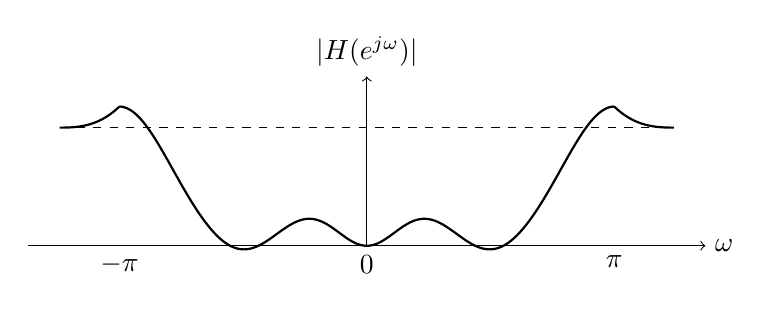
\begin{tikzpicture}[x=1cm,y=1cm]

% 参数
\pgfmathsetmacro{\A}{1.5}
\pgfmathsetmacro{\P}{3.1416}

% 主函数在 x=pi 处的函数值（用于左右两段精确接上）
\pgfmathsetmacro{\Ypi}{
    (1-exp(-0.95*\P*\P)) *
    (
      1.55*(0.18 + 0.82*(cos(deg(\P))*cos(deg(\P))))
      + 0.22*(cos(deg(2*\P))*cos(deg(2*\P)))
      - 0.55*exp(-2.2*(abs(\P)-1.55)^2)
    )
}

% 坐标轴（稍微加长）
\draw[->] (-4.3,0) -- (4.3,0) node[right] {$\omega$};
\draw[->] (0,0) -- (0,2.15) node[above] {$|H(e^{j\omega})|$};

% 横轴标注
\node[below] at (-\P,0) {$-\pi$};
\node[below] at (0,0) {$0$};
\node[below] at (\P,0) {$\pi$};

% 通带参考虚线
\draw[dashed] (-3.9,\A) -- (3.9,\A);

% 左侧延伸平台：改为接到 (-pi, Ypi)
\draw[thick] (-3.9,1.50) .. controls (-3.65,1.50) and (-3.40,1.52) .. (-\P,\Ypi);

% 中间主曲线（-pi 到 pi）——完全保留你的原函数
\draw[thick,domain=-\P:\P,samples=500,smooth]
plot (\x,{
    (1-exp(-0.95*\x*\x)) *
    (
      1.55*(0.18 + 0.82*(cos(deg(\x))*cos(deg(\x))))
      + 0.22*(cos(deg(2*\x))*cos(deg(2*\x)))
      - 0.55*exp(-2.2*(abs(\x)-1.55)^2)
    )
});

% 右侧延伸平台：改为从 (pi, Ypi) 接出去
\draw[thick] (\P,\Ypi) .. controls (3.40,1.52) and (3.65,1.50) .. (3.9,1.50);

\end{tikzpicture}
\end{center}

\vspace{0.5em}
\begin{tabular}{@{}p{0.42\textwidth}p{0.42\textwidth}@{}}
A. 低通滤波器
&
B. 高通滤波器
\\[0.8em]
C. 带通滤波器
&
D. 带阻滤波器
\end{tabular}


\item 某模拟低通滤波器的幅频响应如图所示。根据图中通带与阻带的波动特性及 $\Omega=0$ 处的幅度值，
判断该滤波器的阶数 $N$ 及类型为\blank[1cm]。

\vspace{0.5em}

% 这里插入你找到的图
\begin{figure}[H]
    \centering
    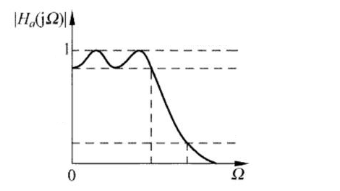
\includegraphics[width=0.35\linewidth]{image/Chebyshev_filter.png}
\end{figure}

\vspace{0.5em}
\begin{tabular}{@{}p{0.42\textwidth}p{0.42\textwidth}@{}}
A. $N=4$，切比雪夫 I 型滤波器
&
B. $N=4$，切比雪夫 II 型滤波器
\\[0.8em]
C. $N=3$，切比雪夫 I 型滤波器
&
D. $N=3$，切比雪夫 II 型滤波器
\end{tabular}

\item 某序列 $x(n)$ 经过插零处理后得到序列 $x_i(n)$，如图所示。由图可知，该插值系统的插值因子 $I$ 及后接理想低通滤波器的通带增益应为（\qquad）。

\begin{center}
\begin{tikzpicture}[x=0.72cm,y=0.9cm]

%==================== 上图 x(n) ====================
\node at (-1.2,4.8) {$x(n)$};
\draw[->] (-0.6,3.2) -- (7.8,3.2) node[right] {$n$};
\draw[->] (0,3.0) -- (0,5.1);

% 上图样值
\foreach \x/\y in {
0/1.25,1/1.75,2/1.10,3/1.55,4/1.30,5/1.65,6/1.05
}{
    \draw[thick] (\x,3.2) -- (\x,{3.2+\y});
    \fill (\x,{3.2+\y}) circle (0.05);
}

% 上图刻度
\foreach \x in {0,1,2,3,4,5,6}
{
    \node[below] at (\x,3.2) {\small $\x$};
}

%==================== 下图 x_i(n) ====================
\node at (-1.2,1.7) {$x_i(n)$};
\draw[->] (-0.6,0) -- (20.8,0) node[right] {$n$};
\draw[->] (0,-0.2) -- (0,2.2);

% 下图非零样值（每隔 3 个点一个）
\foreach \x/\y in {
0/1.25,3/1.75,6/1.10,9/1.55,12/1.30,15/1.65,18/1.05
}{
    \draw[thick] (\x,0) -- (\x,\y);
    \fill (\x,\y) circle (0.05);
}

% 下图插入的零值（画成轴上的小点和极短竖线）
\foreach \x in {1,2,4,5,7,8,10,11,13,14,16,17}
{
    \draw[thick] (\x,0) -- (\x,0.06);
    \fill (\x,0) circle (0.035);
}

% 下图刻度
\foreach \x in {0,1,2,3,4,5,6,7,8,9,10,11,12,13,14,15,16,17,18}
{
    \node[below] at (\x,0) {\scriptsize $\x$};
}

\end{tikzpicture}
\end{center}

\vspace{0.6em}

\begin{tabular}{@{}p{0.42\textwidth}p{0.42\textwidth}@{}}
A. $I=3$，低通滤波器通带增益为 $\dfrac{1}{3}$
&
B. $I=3$，低通滤波器通带增益为 $3$
\\[0.8em]
C. $I=2$，低通滤波器通带增益为 $\dfrac{1}{2}$
&
D. $I=2$，低通滤波器通带增益为 $3$
\end{tabular}


\end{enumerate}

\noindent
\begin{minipage}[t]{0.25\textwidth}
\renewcommand{\arraystretch}{1.5}
\begin{tabular}{|C{1.5cm}|C{2.3cm}|}
\hline
得分 & 评卷人 \\
\hline
\rule{0pt}{0.8cm}&  \\
\hline
\end{tabular}
\end{minipage}
\begin{minipage}[t]{0.72\textwidth}
\vspace{0.2cm}
\begin{center}
{\heiti 三、简答题（共 18 分）}
\end{center}
\end{minipage}

\vspace{1.2em}

\begin{enumerate}[label=\arabic*., leftmargin=2em, itemsep=1.2em]

\item 利用 DFT 进行连续时间信号频谱分析时会产生哪三种误差？产生误差的原因分别是什么？如何减小这三种误差？

\newpage

\vspace*{4cm}

\item 写出用一次 $N$ 点 DFT 计算一个 $2N$ 点实数序列 $x(n)$ 的 DFT 的过程，并写出表达式。

\vspace*{5.5cm}

\item 有一调幅信号 $x_a(t) = [1 + \cos(2\pi \times 50t)] \cos(2\pi \times 500t)$，用 DFT 做频谱分析，要求能分
辨 $x_a(t)$ 的所有频率分量，试确定以下各参数：

(1) 最小记录时间； (2) 最大取样间隔； (3) 最少采样点数；

\vspace*{5.5cm}

\end{enumerate}

\newpage

\noindent
\begin{minipage}[t]{0.25\textwidth}
\renewcommand{\arraystretch}{1.5}
\begin{tabular}{|C{1.5cm}|C{2.3cm}|}
\hline
得分 & 评卷人 \\
\hline
\rule{0pt}{0.8cm}&  \\
\hline
\end{tabular}
\end{minipage}
\begin{minipage}[t]{0.72\textwidth}
\vspace{0.2cm}
\begin{center}
{\heiti 四、（共 12 分）}
\end{center}
\end{minipage}

\vspace{1.2em}

\begin{enumerate}[label={}, leftmargin=2em, itemsep=1.6em]

\item 已知 $x(n)=\delta(n)+\delta(n-2)+2\delta(n-3)$，其 $4$ 点$\mathrm{DFT}$变换为
$X(k)$，试求：

\vspace{0.6em}

（1）若$A(k)=\Re[X(k)],$求$a(n)=\mathrm{IDFT}_4\{A(k)\};$


\vspace{0.6em}

（2）若 $\displaystyle Y(k)=(-1)^kX(k)$，
求 $\displaystyle y(n)$；

\vspace{0.6em}

（3）若 $\displaystyle Z(k)=A(k)Y(k)$，
求 $\displaystyle z(n)$；

\vspace{0.6em}

（4）$X(n)$ 的 $4$ 点 DFT；

\vspace{0.6em}

（5）$\displaystyle \sum_{k=0}^{3}\left|X(k)\right|^2$。

\vspace{6cm}

\end{enumerate}

\noindent
\begin{minipage}[t]{0.25\textwidth}
\renewcommand{\arraystretch}{1.5}
\begin{tabular}{|C{1.5cm}|C{2.3cm}|}
\hline
得分 & 评卷人 \\
\hline
\rule{0pt}{0.8cm}&  \\
\hline
\end{tabular}
\end{minipage}
\begin{minipage}[t]{0.72\textwidth}
\vspace{0.2cm}
\begin{center}
{\heiti 五、（共 8 分）}
\end{center}
\end{minipage}

\vspace{1.2em}

\begin{enumerate}[label={}, leftmargin=2em, itemsep=1.6em]

\item 已知二阶 IIR 数字滤波器的系统函数为
\[
H(z)
=\frac{b_0+b_1z^{-1}+b_2z^{-2}}
{1-a_1z^{-1}-a_2z^{-2}},
\]
试画出该系统的直接 II 型结构图，并写出其对应的差分方程。
\newpage

\vspace*{3cm}

\end{enumerate}


\noindent
\begin{minipage}[t]{0.25\textwidth}
\renewcommand{\arraystretch}{1.5}
\begin{tabular}{|C{1.5cm}|C{2.3cm}|}
\hline
得分 & 评卷人 \\
\hline
\rule{0pt}{0.8cm}&  \\
\hline
\end{tabular}
\end{minipage}
\begin{minipage}[t]{0.72\textwidth}
\vspace{0.2cm}
\begin{center}
{\heiti 六、（共 8 分）}
\end{center}
\end{minipage}

\vspace{1.2em}

\begin{enumerate}[label={}, leftmargin=2em, itemsep=1.6em]

\item 已知一个非周期连续时间信号 $x(t)$，以采样频率
$f_s=1000\,\mathrm{Hz}$ 对其进行等间隔采样，取连续 $100$ 个采样点得到有限长序列
$x_1(n)$。对 $x_1(n)$ 作 $100$ 点 DFT，得到 $X_1(k)$。
将 $x_1(n)$ 末尾补 $28$ 个零，得到 $128$ 点序列 $x_2(n)$，
对 $x_2(n)$ 作 $128$ 点 DFT，得到 $X_2(k)$。试求：

（1）$x_1(n)$ 对应的频谱分辨率。

（2）$X_1(k)$ 中 $k=20$ 点对应的原连续信号频率为多少 Hz？

（3）$x_2(n)$ 对应的频谱分辨率。

（4）$X_2(k)$ 中 $k=20$ 点对应的原连续信号频率为多少 Hz？

\end{enumerate}

\vspace*{4cm}

\noindent
\begin{minipage}[t]{0.25\textwidth}
\renewcommand{\arraystretch}{1.5}
\begin{tabular}{|C{1.5cm}|C{2.3cm}|}
\hline
得分 & 评卷人 \\
\hline
\rule{0pt}{0.8cm}&  \\
\hline
\end{tabular}
\end{minipage}
\begin{minipage}[t]{0.72\textwidth}
\vspace{0.2cm}
\begin{center}
{\heiti 七、（共 10 分）}
\end{center}
\end{minipage}

\vspace{1.2em}

\begin{enumerate}[label={}, leftmargin=2em, itemsep=1.6em]

\item 已知 FIR 系统的系统函数为$H_0(z)=\left(1+z^{-1}+0.25z^{-2}\right)^2$。试求具有相同幅度响应的线性相位 FIR 的单位冲激响应 $h(n)$ 并画出该线性相位 FIR 系统的结构图，并写出该系统对应的差分方程。
\vspace{0.6em}

\newpage

\vspace*{2cm}

\end{enumerate}

\noindent
\begin{minipage}[t]{0.25\textwidth}
\renewcommand{\arraystretch}{1.5}
\begin{tabular}{|C{1.5cm}|C{2.3cm}|}
\hline
得分 & 评卷人 \\
\hline
\rule{0pt}{0.8cm}&  \\
\hline
\end{tabular}
\end{minipage}
\begin{minipage}[t]{0.72\textwidth}
\vspace{0.2cm}
\begin{center}
{\heiti 八、（共10分）}
\end{center}
\end{minipage}

\vspace{1.2em}

\begin{enumerate}[label={}, leftmargin=2em, itemsep=1.6em]

\item 采用双线性变换法设计巴特沃斯数字高通滤波器。已知数字高通滤波器的技术指标为：
通带边界频率 $\omega_p=0.6\pi$，通带最大衰减 $\delta_p=3\,\mathrm{dB}$；
阻带边界频率 $\omega_s=0.4\pi$，阻带最小衰减 $\delta_s=15\,\mathrm{dB}$。
设采样周期 $T=1$。试求：

（1）将上述数字高通滤波器指标转换为等效数字低通滤波器指标。

（已知数字低通到数字高通的频率变换为
$
z^{-1}=F(Z^{-1})
=-\frac{Z^{-1}+\alpha}{1+\alpha Z^{-1}},
$
其中
$
\alpha
=
-\frac{
\cos\left[\dfrac{\theta_c+\omega_c}{2}\right]
}{
\cos\left[\dfrac{\theta_c-\omega_c}{2}\right]
}.
$）


（2）由数字低通滤波器指标求模拟低通滤波器指标。

（3）求巴特沃斯模拟低通滤波器的阶数 $N$。

巴特沃斯低通滤波器阶数
$
N\geq
\frac{
\lg\left[
\dfrac{10^{0.1\delta_s}-1}{10^{0.1\delta_p}-1}
\right]
}{
2\lg\left(\dfrac{\Omega_s}{\Omega_p}\right)
}.
$
预畸变为
$
\Omega=\frac{2}{T}\tan\frac{\omega}{2}.
$

\newpage


\end{enumerate}

\noindent
\begin{minipage}[t]{0.25\textwidth}
\renewcommand{\arraystretch}{1.5}
\begin{tabular}{|C{1.5cm}|C{2.3cm}|}
\hline
得分 & 评卷人 \\
\hline
\rule{0pt}{0.8cm}&  \\
\hline
\end{tabular}
\end{minipage}
\begin{minipage}[t]{0.72\textwidth}
\vspace{0.2cm}
\begin{center}
{\heiti 九、（共8分）}
\end{center}
\end{minipage}

\vspace{1.2em}

\begin{enumerate}[label={}, leftmargin=2em, itemsep=1.6em]

\item 采用窗函数法设计线性相位 FIR 数字低通滤波器。已知通带边界频率
$f_p=150\,\mathrm{Hz}$，阻带边界频率 $f_{st}=250\,\mathrm{Hz}$，
要求阻带相对幅度不高于 $-50\,\mathrm{dB}$，采样频率为
$f_s=1000\,\mathrm{Hz}$。要求在满足指标的前提下，滤波器长度尽可能短。

常用窗函数的性能指标如下表所示：

\begin{center}
\setlength{\tabcolsep}{10pt}
\renewcommand{\arraystretch}{1.7}
\begin{tabular}{c|c|c|c}
\hline
窗函数 & 旁瓣峰值 / dB & 阻带相对幅度 / dB & 过渡带宽 $\Delta\omega$ 近似值 \\
\hline
矩形窗 & $-13$ & $-21$ & $\dfrac{1.8\pi}{N}$ \\
汉宁窗 & $-31$ & $-44$ & $\dfrac{6.2\pi}{N}$ \\
海明窗 & $-41$ & $-53$ & $\dfrac{6.6\pi}{N}$ \\
布莱克曼窗 & $-57$ & $-74$ & $\dfrac{11\pi}{N}$ \\
\hline
\end{tabular}
\end{center}

试求：

（1）应选用哪种窗函数；

（2）滤波器长度 $N$ 至少应取多少；

（3）该滤波器的阶数；

（4）该滤波器的延迟时间。

\newpage


\end{enumerate}




\newpage

\begin{center}
{\heiti\zihao{3} 参考答案}
\end{center}

\vspace{1em}

\begingroup
\small
\setlength{\parskip}{0.25em}

\section*{一、填空题}

\begin{enumerate}[label=\arabic*., leftmargin=2em]
\item $\omega=\dfrac{2\pi}{5}$；周期为 $5$。
\item 直接计算：$N^2 = 900$ 次；$30$ 点不能直接采用基-$2$ FFT。若补零到 $32$ 点，复数乘法为
\[
\frac{32}{2}\log_2 32=80.
\]
\item $L+M-1$；$M-1$。
\item $\{\underline{7},2,2,1,1\}$。。
\item 
若课程采用 $h(n)=T h_a(nT)$，则为
\[
H(z)=\frac{T}{1-e^{-2T}z^{-1}}.
\]
\end{enumerate}

\section*{二、单选题}

\[
\boxed{1.\ D \qquad 2.\ A \qquad 3.\ B \qquad 4.\ A \qquad 5.\ B}
\]

\section*{三、简答题}

\begin{enumerate}[label=\arabic*., leftmargin=2em]

\item 三种误差为：混叠误差、泄漏误差和栅栏效应。

混叠误差：采样频率不满足采样定理，$f_s<2f_h$。减小方法：提高采样频率，并在采样前加抗混叠低通滤波器。

泄漏误差：实际只能截取有限长信号，相当于加窗，频域发生卷积。减小方法：增加记录长度，或选用合适窗函数。

栅栏效应：DFT 只在有限个离散频率点上取样，真实频率分量可能不落在谱线点上。减小方法：增加 DFT 点数或补零，使频率采样点更密。补零不能提高实际物理分辨率。

\item 构造 $N$ 点复序列
\[
y(n)=x(2n)+jx(2n+1),\quad n=0,1,\cdots,N-1.
\]
\[
Y(k)=\mathrm{DFT}_N\{y(n)\}.
\]
\[
A(k)=\frac{1}{2}\left[Y(k)+Y^*((N-k)_N)\right],
\]
\[
B(k)=\frac{1}{2j}\left[Y(k)-Y^*((N-k)_N)\right].
\]
则原 $2N$ 点实序列的 DFT 为
\[
X(k)=A((k)_N)+W_{2N}^{k}B((k)_N),
\quad k=0,1,\cdots,2N-1.
\]

\item
已知
\[
x_a(t)=[1+\cos(2\pi\times 50t)]\cos(2\pi\times 500t).
\]

利用积化和差公式：
\[
x_a(t)=\cos(2\pi\times500t)
+\frac12\cos(2\pi\times550t)
+\frac12\cos(2\pi\times450t).
\]

因此频率分量为
\[
450\,\mathrm{Hz},\quad 500\,\mathrm{Hz},\quad 550\,\mathrm{Hz}.
\]

相邻频率分量间隔为 $50\,\mathrm{Hz}$，所以最小记录时间为
\[
T_{\min}=\frac{1}{50}=0.02\,\mathrm{s}.
\]

最高频率为 $550\,\mathrm{Hz}$，由采样定理：
\[
f_s\geq 2\times550=1100\,\mathrm{Hz}.
\]

所以最大取样间隔为
\[
T_s\leq \frac{1}{1100}\,\mathrm{s}.
\]

最少采样点数为
\[
N\geq T_{\min}f_s
=0.02\times1100
=22.
\]

\end{enumerate}

\section*{四、DFT 性质综合题}

已知
\[
x(n)=\delta(n)+\delta(n-2)+2\delta(n-3)
=\{\underline{1},0,1,2\}.
\]
其 $4$ 点 DFT 为
\[
X(k)=\{4,\ 2j,\ 0,\ -2j\}.
\]

\begin{enumerate}[label=（\arabic*）, leftmargin=2.5em]

\item
\[
A(k)=\Re[X(k)]=\{4,0,0,0\},
\]
\[
a(n)=\mathrm{IDFT}_4\{A(k)\}
=\{\underline{1},1,1,1\}.
\]

\item
\[
Y(k)=(-1)^kX(k)=W_4^{-2k}X(k),
\]
故
\[
y(n)=x((n+2))_4=\{\underline{1},2,1,0\}.
\]

\item
\[
z(n)=a(n)\circledast_4 y(n).
\]
由于
\[
a(n)=\{\underline{1},1,1,1\},
\quad
y(n)=\{\underline{1},2,1,0\},
\]
故
\[
z(n)=\{\underline{4},4,4,4\}.
\]

\item 由 DFT 对偶性：
\[
\mathrm{DFT}_4\{X(n)\}=4x((-k)_4)
=\{\underline{4},8,4,0\}.
\]

\item 由 Parseval 定理：
\[
\sum_{k=0}^{3}|X(k)|^2
=
4\sum_{n=0}^{3}|x(n)|^2
=
4(1^2+0^2+1^2+2^2)=24.
\]

\end{enumerate}

\section*{五、IIR 结构题}

引入中间变量 $w(n)$，直接 II 型可写为
\[
w(n)=x(n)+a_1w(n-1)+a_2w(n-2),
\]
\[
y(n)=b_0w(n)+b_1w(n-1)+b_2w(n-2).
\]

因此结构图为：输入 $x(n)$ 先经过两级反馈延时形成 $w(n)$，再经 $b_0,b_1,b_2$ 三个前馈支路相加得到 $y(n)$，共用两个单位延时器。

由
\[
H(z)=
\frac{b_0+b_1z^{-1}+b_2z^{-2}}
{1-a_1z^{-1}-a_2z^{-2}},
\]
得差分方程：
\[
\boxed{
y(n)=a_1y(n-1)+a_2y(n-2)
+b_0x(n)+b_1x(n-1)+b_2x(n-2)
}.
\]

\section*{六、频谱分辨率题}

已知
\[
f_s=1000\,\mathrm{Hz}.
\]

\[
T_1=\frac{100}{1000}=0.1\,\mathrm{s},
\qquad
\Delta f_{\mathrm{phys}}=\frac{1}{T_1}=10\,\mathrm{Hz}.
\]

（1）
\[
\boxed{10\,\mathrm{Hz}}
\]

（2）
\[
f_1(20)=20\cdot\frac{1000}{100}=200\,\mathrm{Hz}.
\]

（3）补零后实际记录时间不变，因此实际物理分辨率仍为
\[
\boxed{10\,\mathrm{Hz}}.
\]
但 $128$ 点 DFT 的频率间隔为
\[
\Delta f_2=\frac{1000}{128}=7.8125\,\mathrm{Hz}.
\]

（4）
\[
f_2(20)=20\cdot\frac{1000}{128}=156.25\,\mathrm{Hz}.
\]

补零只使频率采样点变密，不提高实际物理分辨率。

\section*{七、FIR 线性相位结构题}

\[
H_0(z)=\left(1+z^{-1}+0.25z^{-2}\right)^2.
\]

令
\[
D(z)=1+z^{-1}+0.25z^{-2},
\]
其镜像多项式为
\[
D_r(z)=0.25+z^{-1}+z^{-2}.
\]

取
\[
H(z)=D(z)D_r(z).
\]

则
\[
H(z)=
\left(1+z^{-1}+0.25z^{-2}\right)
\left(0.25+z^{-1}+z^{-2}\right).
\]

展开得
\[
H(z)=0.25+1.25z^{-1}+2.0625z^{-2}+1.25z^{-3}+0.25z^{-4}.
\]

所以
\[
h(n)=\{\underline{0.25},1.25,2.0625,1.25,0.25\}.
\]

差分方程为
\[
y(n)=0.25x(n)+1.25x(n-1)+2.0625x(n-2)+1.25x(n-3)+0.25x(n-4).
\]

按线性相位结构可写为
\[
y(n)=0.25[x(n)+x(n-4)]
+1.25[x(n-1)+x(n-3)]
+2.0625x(n-2).
\]

结构图画法：$x(n)$ 经 $4$ 个单位延时器形成 $x(n)$ 到 $x(n-4)$，两端对称相加后分别乘 $0.25$、$1.25$，中间项 $x(n-2)$ 乘 $2.0625$，三路相加得到 $y(n)$。

\section*{八、巴特沃斯数字高通滤波器设计}

已知
\[
\omega_p=0.6\pi,\quad \omega_s=0.4\pi,
\quad
\delta_p=3\,\mathrm{dB},\quad \delta_s=15\,\mathrm{dB}.
\]

（1）等效数字低通指标：
\[
\theta_p=\pi-\omega_p=0.4\pi,
\qquad
\theta_s=\pi-\omega_s=0.6\pi.
\]
故
\[
\boxed{\theta_p=0.4\pi,\quad \theta_s=0.6\pi}.
\]

由题给公式取
\[
\theta_c=0.4\pi,\quad \omega_c=0.6\pi,
\]
得
\[
\alpha
=
-\frac{\cos(0.5\pi)}{\cos(-0.1\pi)}
=0.
\]

（2）预畸变：
\[
\Omega=\frac{2}{T}\tan\frac{\theta}{2},\quad T=1.
\]
所以
\[
\Omega_p=2\tan(0.2\pi)\approx 1.453,
\]
\[
\Omega_s=2\tan(0.3\pi)\approx 2.753.
\]

（3）阶数：
\[
N\geq
\frac{
\lg\left[
\dfrac{10^{0.1\delta_s}-1}{10^{0.1\delta_p}-1}
\right]
}{
2\lg\left(\dfrac{\Omega_s}{\Omega_p}\right)
}
\approx
\frac{1.488}{0.555}
\approx 2.68.
\]
故
\[
\boxed{N=3}.
\]

\section*{九、FIR 窗函数法设计}

\[
\Delta f=f_{st}-f_p=250-150=100\,\mathrm{Hz}.
\]
\[
\Delta\omega=
2\pi\frac{\Delta f}{f_s}
=
2\pi\frac{100}{1000}
=
0.2\pi.
\]

阻带相对幅度要求不高于 $-50\,\mathrm{dB}$。汉宁窗 $-44\,\mathrm{dB}$ 不满足，海明窗 $-53\,\mathrm{dB}$ 满足，且比布莱克曼窗长度短。

故选
\[
\boxed{\text{海明窗}}.
\]

海明窗：
\[
\Delta\omega\approx \frac{6.6\pi}{N}.
\]
因此
\[
N\geq \frac{6.6\pi}{0.2\pi}=33.
\]
所以
\[
\boxed{N=33}.
\]

阶数：
\[
\boxed{N-1=32}.
\]

群延迟：
\[
\tau=\frac{N-1}{2}=16
\]
个采样点。由于
\[
T=\frac{1}{1000}=0.001\,\mathrm{s},
\]
所以延迟时间为
\[
\boxed{16T=0.016\,\mathrm{s}}.
\]

\endgroup

\end{document}
